% Intended LaTeX compiler: pdflatex
\documentclass[presentation,aspectratio=169]{beamer}
\usepackage[utf8]{inputenc}
\usepackage[T1]{fontenc}
\usepackage{graphicx}
\usepackage{grffile}
\usepackage{longtable}
\usepackage{wrapfig}
\usepackage{rotating}
\usepackage[normalem]{ulem}
\usepackage{amsmath}
\usepackage{textcomp}
\usepackage{amssymb}
\usepackage{capt-of}
\usepackage{hyperref}
\setbeamertemplate{navigation symbols}{}
\usepackage{ebgaramond}
\usefonttheme{serif}
\usetheme{Pittsburgh}
\setbeamertemplate{caption}[numbered]
\setbeamertemplate{caption label separator}{: }
\setbeamercolor{caption name}{fg=normal text.fg}
\usepackage{amsmath,amssymb}
\usepackage{textpos}
\usetheme{default}
\author{Frank Terbeck\thanks{ft@bewatermyfriend.org}}
\date{\today}
\title{C \(\not\subset\) C++}
\author{\texorpdfstring{Frank Terbeck\newline\tiny{\url{ft@bewatermyfriend.org}}}{Frank Terbeck}}
\AtBeginSection{\let\insertsectionnumber\relax \let\sectionname\relax \frame{\sectionpage}}
\hypersetup{
 pdfauthor={Frank Terbeck},
 pdftitle={C \(\not\subset\) C++},
 pdfkeywords={C C++ Standards Subset},
 pdfsubject={},
 pdflang={English}}
\begin{document}

\maketitle

\begin{frame}[label={sec:org2cd0672}]{C \(\subset\) C++ — Right!?}
\begin{center}
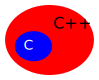
\includegraphics[width=0.5\textwidth]{./graphics/csubset.pdf}
\end{center}
\end{frame}

\section{In Reality: C \(\not\subset\) C++}
\label{sec:orgf0e5bbb}

%%%%%%%%%%%%%%%%%%%%%%%%%%%%%%%%%%%%%%%%%%%%%%%%%%%%%%%%%%%%%%%%%%%%%%%%%%%%%%%

\begin{frame}[fragile,label={sec:orgb26de58}]{Quiz — \texttt{main()}}
 \begin{columns}
\begin{column}{0.48\columnwidth}
\begin{block}{Code}
\begin{verbatim}
main(void)
{
    /* ... */
}
\end{verbatim}
\end{block}
\end{column}

\begin{column}{0.48\columnwidth}
\begin{block}{Questions}
\begin{itemize}
\item Valid C?
\item Valid C++?
\item Both?
\item Neither!?
\end{itemize}
\end{block}
\end{column}
\end{columns}

\begin{block}<2>{C}
\begin{verbatim}
test.c:1:1: warning: return type defaults to ‘int’ [-Wimplicit-int]
\end{verbatim}
``Implicit \texttt{int}'' should be an error since \texttt{C99}: \texttt{ -Werror-implicit-int}
\end{block}

\vspace{-2cm}

\begin{block}<3>{C++}
\begin{verbatim}
test.cpp:1:10: warning: ISO C++ forbids declaration of ‘main’ with
               no type [-Wreturn-type]
\end{verbatim}
\end{block}
\end{frame}

%%%%%%%%%%%%%%%%%%%%%%%%%%%%%%%%%%%%%%%%%%%%%%%%%%%%%%%%%%%%%%%%%%%%%%%%%%%%%%%

\begin{frame}[fragile,label={sec:org1921130}]{Quiz — Data}
 \begin{columns}
\begin{column}{0.48\columnwidth}
\begin{block}{Code}
\begin{verbatim}
struct FooBar {
    int a;
    int b;
};
/* ... */
Foobar fb;
\end{verbatim}
\end{block}
\end{column}

\begin{column}{0.48\columnwidth}
\begin{block}{Questions}
\begin{itemize}
\item Valid C?
\item Valid C++?
\item Both?
\item Neither!?
\end{itemize}

\vspace{0.5cm}
\end{block}
\end{column}
\end{columns}
\begin{block}<2>{C}
\begin{verbatim}
test.c:9:5: error: unknown type name ‘FooBar’; use ‘struct’ keyword
            to refer to the type
\end{verbatim}

\begin{verbatim}
typedef struct FooBar { int a; int b; } FooBar;
\end{verbatim}
\end{block}
\end{frame}

%%%%%%%%%%%%%%%%%%%%%%%%%%%%%%%%%%%%%%%%%%%%%%%%%%%%%%%%%%%%%%%%%%%%%%%%%%%%%%%

\begin{frame}[fragile,label={sec:org23c4234}]{Quiz — \texttt{auto}}
 \begin{columns}
\begin{column}{0.48\columnwidth}
\begin{block}{Code}
\begin{verbatim}
  auto x = 2.25;
\end{verbatim}
\end{block}
\end{column}

\begin{column}{0.48\columnwidth}
\begin{block}{Questions}
\begin{itemize}
\item Valid C?
\item Valid C++?
\item Both?
\item Neither!?
\end{itemize}
\end{block}
\end{column}
\end{columns}

\begin{block}<2>{C}
\begin{verbatim}
test.c:4:10: warning: type defaults to ‘int’ in declaration of
             ‘x’ [-Wimplicit-int]
test.c:4:14: warning: implicit conversion from 'double' to 'int'
             changes value from 2.25 to 2 [-Wliteral-conversion]
\end{verbatim}

\end{block}
\vspace{-3cm}
\begin{block}<3>{C++}
From \texttt{C++11} \texttt{x} will be a \texttt{double} via type inference.
\end{block}
\end{frame}

%%%%%%%%%%%%%%%%%%%%%%%%%%%%%%%%%%%%%%%%%%%%%%%%%%%%%%%%%%%%%%%%%%%%%%%%%%%%%%%

\begin{frame}[fragile,label={sec:org23c4234}]{Quiz — \texttt{auto}, Part II}
 \begin{columns}
\begin{column}{0.48\columnwidth}
\begin{block}{Code}
\begin{verbatim}
  auto int y = 5;
\end{verbatim}
\end{block}
\end{column}

\begin{column}{0.48\columnwidth}
\begin{block}{Questions}
\begin{itemize}
\item Valid C?
\item Valid C++?
\item Both?
\item Neither!?
\end{itemize}
\end{block}
\end{column}
\end{columns}

\begin{block}<2>{C}

Valid C.

\end{block}
\vspace{-1cm}
\begin{block}<3>{C++}
\begin{verbatim}
test.cpp:4:14: error: two or more data types in declaration of ‘y’

test.cpp:4:5: warning: 'auto' storage class specifier is not permit-
              ted in C++11, and will not be supported in future re-
              leases [-Wauto-storage-class]
\end{verbatim}
\end{block}
\end{frame}

%%%%%%%%%%%%%%%%%%%%%%%%%%%%%%%%%%%%%%%%%%%%%%%%%%%%%%%%%%%%%%%%%%%%%%%%%%%%%%%

\begin{frame}[fragile,label={sec:org23c4234}]{Quiz — \texttt{auto}, Part II}
 \begin{columns}
\begin{column}{0.48\columnwidth}
\begin{block}{Code}
\begin{verbatim}
  register int z = 5;
\end{verbatim}
\end{block}
\end{column}

\begin{column}{0.48\columnwidth}
\begin{block}{Questions}
\begin{itemize}
\item Valid C?
\item Valid C++?
\item Both?
\item Neither!?
\end{itemize}
\end{block}
\end{column}
\end{columns}

\begin{block}<2>{C}

Valid C.

\end{block}
\vspace{-1cm}
\begin{block}<3>{C++}
\begin{verbatim}
test.cpp:4:5: error: ISO C++17 does not allow 'register' storage
              class specifier [-Wregister]
\end{verbatim}
\end{block}
\end{frame}

%%%%%%%%%%%%%%%%%%%%%%%%%%%%%%%%%%%%%%%%%%%%%%%%%%%%%%%%%%%%%%%%%%%%%%%%%%%%%%%

\begin{frame}[fragile,label={sec:org23c4234}]{Quiz — VLA}
 \begin{columns}
\begin{column}{0.48\columnwidth}
\begin{block}{Code}
\begin{verbatim}
  int x = 8;
  int a[x];
\end{verbatim}
\end{block}
\end{column}

\begin{column}{0.48\columnwidth}
\begin{block}{Questions}
\begin{itemize}
\item Valid C?
\item Valid C++?
\item Both?
\item Neither!?
\end{itemize}
\end{block}
\end{column}
\end{columns}

\begin{block}<2>{C}
\begin{itemize}
\item Valid C (since \texttt{C99}): Variable Length Arrays.
\item Optional since \texttt{C11}.
\item Also: ``USING VLAs IS ACTIVELY STUPID!'' -- Linus T.
\end{itemize}
\end{block}

\vspace{-2cm}
\begin{block}<3>{C++}
\begin{verbatim}
test.cpp:5:10: warning: variable length arrays are a C99
              feature [-Wvla-extension]
\end{verbatim}
\end{block}
\end{frame}

%%%%%%%%%%%%%%%%%%%%%%%%%%%%%%%%%%%%%%%%%%%%%%%%%%%%%%%%%%%%%%%%%%%%%%%%%%%%%%%

\begin{frame}[fragile,label={sec:org23c4234}]{Quiz — Initialisation}
 \begin{columns}
\begin{column}{0.48\columnwidth}
\begin{block}{Code}
\begin{verbatim}
  FooBar fb = { .b = 1,
                .a = 2 };
\end{verbatim}
\end{block}
\end{column}

\begin{column}{0.48\columnwidth}
\begin{block}{Questions}
\begin{itemize}
\item Valid C?
\item Valid C++?
\item Both?
\item Neither!?
\end{itemize}
\end{block}
\end{column}
\end{columns}

\begin{block}<2>{C}
Valid C (since \texttt{C99}): Designated Initialisers
\end{block}

\vspace{-1cm}
\begin{block}<3>{C++}
\begin{verbatim}
test.cpp:6:41: error: designator order for field ‘FooBar::a’ does
               not match declaration order in ‘FooBar’
\end{verbatim}
\end{block}
\end{frame}

%%%%%%%%%%%%%%%%%%%%%%%%%%%%%%%%%%%%%%%%%%%%%%%%%%%%%%%%%%%%%%%%%%%%%%%%%%%%%%%

\begin{frame}[fragile,label={sec:org23c4234}]{Quiz — Newer C Features}
 \begin{columns}
\begin{column}{0.48\columnwidth}
\begin{block}{Code}
\begin{verbatim}
  _Atomic char f = 'f';
  _Bool g = true;
\end{verbatim}
\end{block}
\end{column}

\begin{column}{0.48\columnwidth}
\begin{block}{Questions}
\begin{itemize}
\item Valid C?
\item Valid C++?
\item Both?
\item Neither!?
\end{itemize}
\end{block}
\end{column}
\end{columns}

\begin{block}<2>{C++}
\begin{verbatim}
test.cpp:4:5: error: ‘_Atomic’ was not declared in this scope
test.cpp:5:5: error: ‘_Bool’ was not declared in this scope
\end{verbatim}
\end{block}
\end{frame}

%%%%%%%%%%%%%%%%%%%%%%%%%%%%%%%%%%%%%%%%%%%%%%%%%%%%%%%%%%%%%%%%%%%%%%%%%%%%%%%

\begin{frame}[fragile,label={sec:org23c4234}]{Quiz — Newer C Features}
 \begin{columns}
\begin{column}{0.48\columnwidth}
\begin{block}{Code}
\begin{verbatim}
#define cbrt(x)
  _Generic((x),           \
      long double: cbrtl, \
      float: cbrtf        \
      default: cbrt,      \
      )(x)
\end{verbatim}
\end{block}
\end{column}

\begin{column}{0.48\columnwidth}
\begin{block}{Questions}
\begin{itemize}
\item Valid C?
\item Valid C++?
\item Both?
\item Neither!?
\end{itemize}
\end{block}
\end{column}
\end{columns}

\begin{block}<2>{C++}
\begin{verbatim}
test.cpp:8:5: warning: generic selections are a C11-specific
              feature [-Wc11-extensions]
\end{verbatim}
\end{block}
\end{frame}

%%%%%%%%%%%%%%%%%%%%%%%%%%%%%%%%%%%%%%%%%%%%%%%%%%%%%%%%%%%%%%%%%%%%%%%%%%%%%%%

\begin{frame}[fragile,label={sec:org23c4234}]{Quiz — \texttt{void} Conversion}
 \begin{columns}
\begin{column}{0.48\columnwidth}
\begin{block}{Code}
\begin{verbatim}
  int *ii;
  ii = malloc(sizeof(*ii));
\end{verbatim}
\end{block}
\end{column}

\begin{column}{0.48\columnwidth}
\begin{block}{Questions}
\begin{itemize}
\item Valid C?
\item Valid C++?
\item Both?
\item Neither!?
\end{itemize}
\end{block}
\end{column}
\end{columns}

\begin{block}<2>{C++}
\begin{verbatim}
test.cpp:6:21: error: invalid conversion from ‘void*’ to ‘int*’
               [-fpermissive]
\end{verbatim}
\end{block}
\end{frame}

%%%%%%%%%%%%%%%%%%%%%%%%%%%%%%%%%%%%%%%%%%%%%%%%%%%%%%%%%%%%%%%%%%%%%%%%%%%%%%%

\begin{frame}[fragile,label={sec:org23c4234}]{Quiz — Character Literals}
 \begin{columns}
\begin{column}{0.48\columnwidth}
\begin{block}{Code}
\begin{verbatim}
  size_t chlitsize = sizeof('%');
\end{verbatim}
\end{block}
\end{column}

\begin{column}{0.48\columnwidth}
\begin{block}{Questions}
\begin{itemize}
\item Valid C?
\item Valid C++?
\item Both?
\item Neither!?
\end{itemize}
\end{block}
\end{column}
\end{columns}

\begin{block}<2>{C}
In C, a character literal is an \texttt{int}.
\end{block}

\vspace{-1cm}
\begin{block}<3>{C++}
In C, a character literal is a \texttt{char}.
\end{block}
\end{frame}

%%%%%%%%%%%%%%%%%%%%%%%%%%%%%%%%%%%%%%%%%%%%%%%%%%%%%%%%%%%%%%%%%%%%%%%%%%%%%%%

\begin{frame}[fragile,label={sec:org23c4234}]{Quiz — Keywords}
 \begin{columns}
\begin{column}{0.48\columnwidth}
\begin{block}{Code}
\begin{verbatim}
int
main(void)
{
    quux();
}
\end{verbatim}
\end{block}
\end{column}

\begin{column}{0.48\columnwidth}
\begin{block}{Questions}
\begin{itemize}
\item Valid C?
\item Valid C++?
\item Both?
\item Neither!?
\end{itemize}
\end{block}
\end{column}
\end{columns}

\begin{block}<2>{C}
\begin{verbatim}
test.c:4:5: warning: implicit declaration of function ‘quux’
\end{verbatim}
Should be an error since \texttt{C99}: \texttt{ -Werror-implicit-function-declaration}
\end{block}

\vspace{-2cm}
\begin{block}<3>{C++}
\begin{verbatim}
test.cpp:4:5: error: ‘quux’ was not declared in this scope
\end{verbatim}
\end{block}
\end{frame}

%%%%%%%%%%%%%%%%%%%%%%%%%%%%%%%%%%%%%%%%%%%%%%%%%%%%%%%%%%%%%%%%%%%%%%%%%%%%%%%

\begin{frame}[fragile,label={sec:org23c4234}]{Quiz — \texttt{main()} — Part II}
 \begin{columns}
\begin{column}{0.48\columnwidth}
\begin{block}{Code}
\begin{verbatim}
int
main(void)
{
}
\end{verbatim}
\end{block}
\end{column}

\begin{column}{0.48\columnwidth}
\begin{block}{Questions}
\begin{itemize}
\item Valid C?
\item Valid C++?
\item Both?
\item Neither!?
\end{itemize}
\end{block}
\end{column}
\end{columns}

\begin{block}<2>{C}
Valid since \texttt{C99} (to match \texttt{C++} sadly). Before:
\begin{verbatim}
test.c:4:1: warning: control reaches end of non-void function
\end{verbatim}
\end{block}

\vspace{-2cm}
\begin{block}<3>{C++}
Valid \texttt{C++}. Returns \texttt{0}. Only applies to \texttt{main()}.
\end{block}
\end{frame}

%%%%%%%%%%%%%%%%%%%%%%%%%%%%%%%%%%%%%%%%%%%%%%%%%%%%%%%%%%%%%%%%%%%%%%%%%%%%%%%

\begin{frame}[fragile,label={sec:org23c6824}]{Closing Thoughts}
  \begin{itemize}
  \item These are not all differences!
  \item Almost everything is language version dependent.
  \item Almost everything is toolchain dependent.
  \item Idiomatic C is not idiomatic C++
  \item …and visa-versa.
  \item Interfaces are the solution.
  \item Compiling C with a C++ compiler is not.
  \end{itemize}
\end{frame}

%%%%%%%%%%%%%%%%%%%%%%%%%%%%%%%%%%%%%%%%%%%%%%%%%%%%%%%%%%%%%%%%%%%%%%%%%%%%%%%


\section{Thanks for your attention!}
\label{sec:org6df872a}
\end{document}
